\section[Clustering]{Utterance Embedding Clustering \label{method: utterance embedding clustering}}
    \begin{figure}[t]
        \centering
        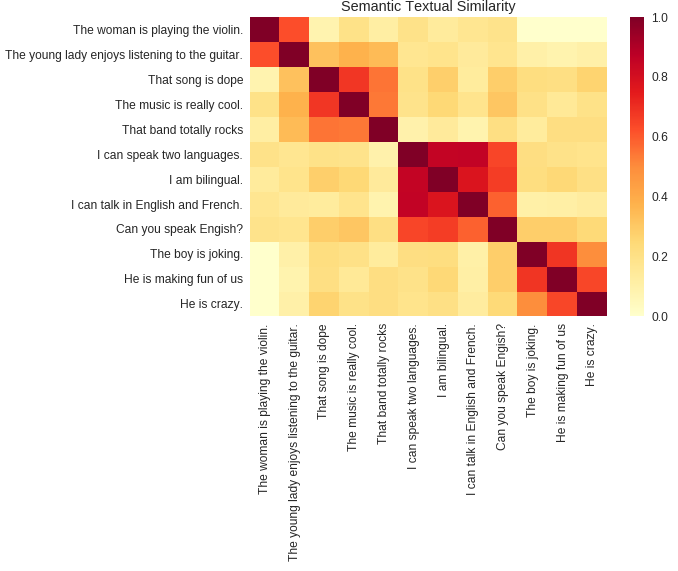
\includegraphics[width=0.8\textwidth]{sentence_similarity.png}
        \caption{Using Google's universal sentence encoder, sentences are embedded and their similarity visualised. The colour of the field at (row, column) indicates the similarity between the sentence labels at (row, column). A darker colour indicates a stronger similarity.}
        \label{fig:sentence similarity}
    \end{figure}
    Using \gls{utterance} \glspl{embedding}, similar sentences can be clustered together, forming topics. Going through the transcript, once the cluster to which a sentence is assigned changes, a topic boundary is set. This theoretically allows for topic segmentation. A visual example showing clusters of similar sentences is shown in Fig. \ref{fig:sentence similarity}.
    
    \subsection{Minimum Cut Graph Based \label{method: minimum cut}}
    
        Firstly we evaluate the minimum cut based clustering method detailed in Sec. \ref{fig: graph seg} for conversations, in which all \glspl{utterance} above some threshold similarity are clustered. The key limitation within the context of conversation is that certain \glspl{utterance} appear within all topics. Consider the following sample of \glspl{utterance}:
        \begin{table}[h]
            \begin{tabular}{l|l}
            $u_1$     & \textit{Rock music is the best!}                        \\
            $u_2$     & \textit{Yeah man, rock is the best!}                    \\
            \dots      &                                                         \\
            $u_i$     & \textit{Lord of the Rings is the best movie ever made.} \\
            $u_{i+1}$ & \textit{Yeah dude, Lord of the Rings really is the best.}              \\
            \end{tabular}
        \end{table}
        
        Even though $u_1$ and $u_{i}$ correctly do not connect, $u_1$ connects to $u_2$, $u_{i}$ connects to $u_{i+1}$ and critically, $u_2$ connects to $u_{i+1}$. This last connection is made because the sentences are similar, in fact everything \textit{except for the topic} matches between these \glspl{utterance}. In conversation, sentences like $u_2$ and $u_{i+1}$ are abundant - leading to one giant connected component, which is a cluster that contains a large fraction of all nodes. We attempted to fine-tune the cutoff similarity, but either (almost) no sentences end up connected or all of them do. 
        
    
    \subsection{Other Clustering Methods}
        Since the cutoff-based approach lead to issues, we try the following clustering methods in an attempt to minimize the vulnerability to falsely merged clusters:
        \begin{itemize}
            \item k-means clustering, in which the algorithm tries to separate samples in k groups of equal variance.
            \item DBSCAN clustering, in which clusters are viewed as areas of high density separated by areas of low density.
            \item Agglomerative clustering, in which a hierarchy of clusters is formed by assigning each \gls{utterance} its own cluster and then repeatedly merging the most similar clusters.
        \end{itemize}
        All three clustering methods were implemented using the python library scikit-learn\cite{scikit-learn}. While some clustering methods (especially agglomerative clustering) qualitatively perform better than the minimum cut method, none work well enough to warrant time-consuming quantitative evaluation.
        
        %These clustering methods qualitatively perform better than the minimum cut method, but each suffer from new issues. In k-means, imposing the number of topics $k$ is difficult as it varies heavily from conversation to conversation. In DBSCAN clustering, which requires neither a cutoff nor a number of topics, if data points are not inherently clustered (i.e. separated by areas of low density), the algorithm fails. This occured for a significant fraction of \glspl{utterance}. The most promising algorithm for clustering was the agglomerative clustering method, in which some topics could be clearly identified, but qualitative results were still too poor to warrant further development and quantitative evaluation.
        
    \subsection{Limitations}
        No matter the clustering method, using sentence embeddings is ineffective when analysing conversation topics. Utterances in casual conversations are more than just their topics, many words dilute the semantics of an \gls{utterance} to such an extent that it becomes 
        \begin{enumerate}
            \item indistinguishable from other \glspl{utterance} talking about different topics
            \item too dissimilar to other utterances talking about the same topic
        \end{enumerate}
        making it a poor method for topic segmentation.
        
        
        %A lot of words Some words in sentences don't contribute to the meaning act as unwanted bridges to other topics, but they can also \textit{dilute} the embedding. Consider the \glspl{utterance}
        
        
        %\begin{table}[h]
        %    \begin{tabular}{l|l}
        %    $u_1$     & \textit{Do you have any pets?}                    \\
        %    $u_2$     & \textit{Yeah, well, we had a light brown cat when I was younger, but I don't now.}                        \\
        %    \end{tabular}
        %\end{table}
        
        %Both \glspl{utterance} are about pets, but because the question and answer share almost no other words, and because the answer is very long, the sentences are deemed dissimilar by the model. %TODO: actually get the sim value
        
        
        
        %The issue with the \gls{utterance} embedding approach can be succinctly summarised as the following: Utterances are more than just their topics. While the similarity of \glspl{utterance} is correlated with the similarity of the topics in which they lie, they are not equivalent. To make a more effective algorithm, the words representing topics must be first extracted.